\section{Monitor electricity consumption}
% Othe purpose, the fact that they have the 'same' client [although I think they are different research groups], and the differences,
Meaningful introduction:
such as the data collection and the target user of the dashboards or project age etc.

\subsection{Initial Hypothesis}\label{sub:vub_initial_hp}
\paragraph{Client} 
% with the motto: \textit{"Conquering darkness by science"} 
\ac{GEP} is a joint project of the \ac{VUB} (Free University of Brussels), dutch and English-speaking research university, and the \ac{UZB} (University Hospital of Brussels), 
which purpose is to develop and operate a research campus in the Research park of Zellik with a focus on the following three research domains:
\begin{itemize}
    \item Energy and mobility transition.
    \item Hospital of the future, part of \ac{BHC}.
    \item Smart regions.
\end{itemize}
With this research campus, Green Energy Park aims to bridge the gap between research, innovation, realization and exploitation, by acting as a large-scale living lab, expertise and training centre~\cite{Misc:vub_2020_green}.
\paragraph{Context Introduction}
\begin{figure}[ht]
    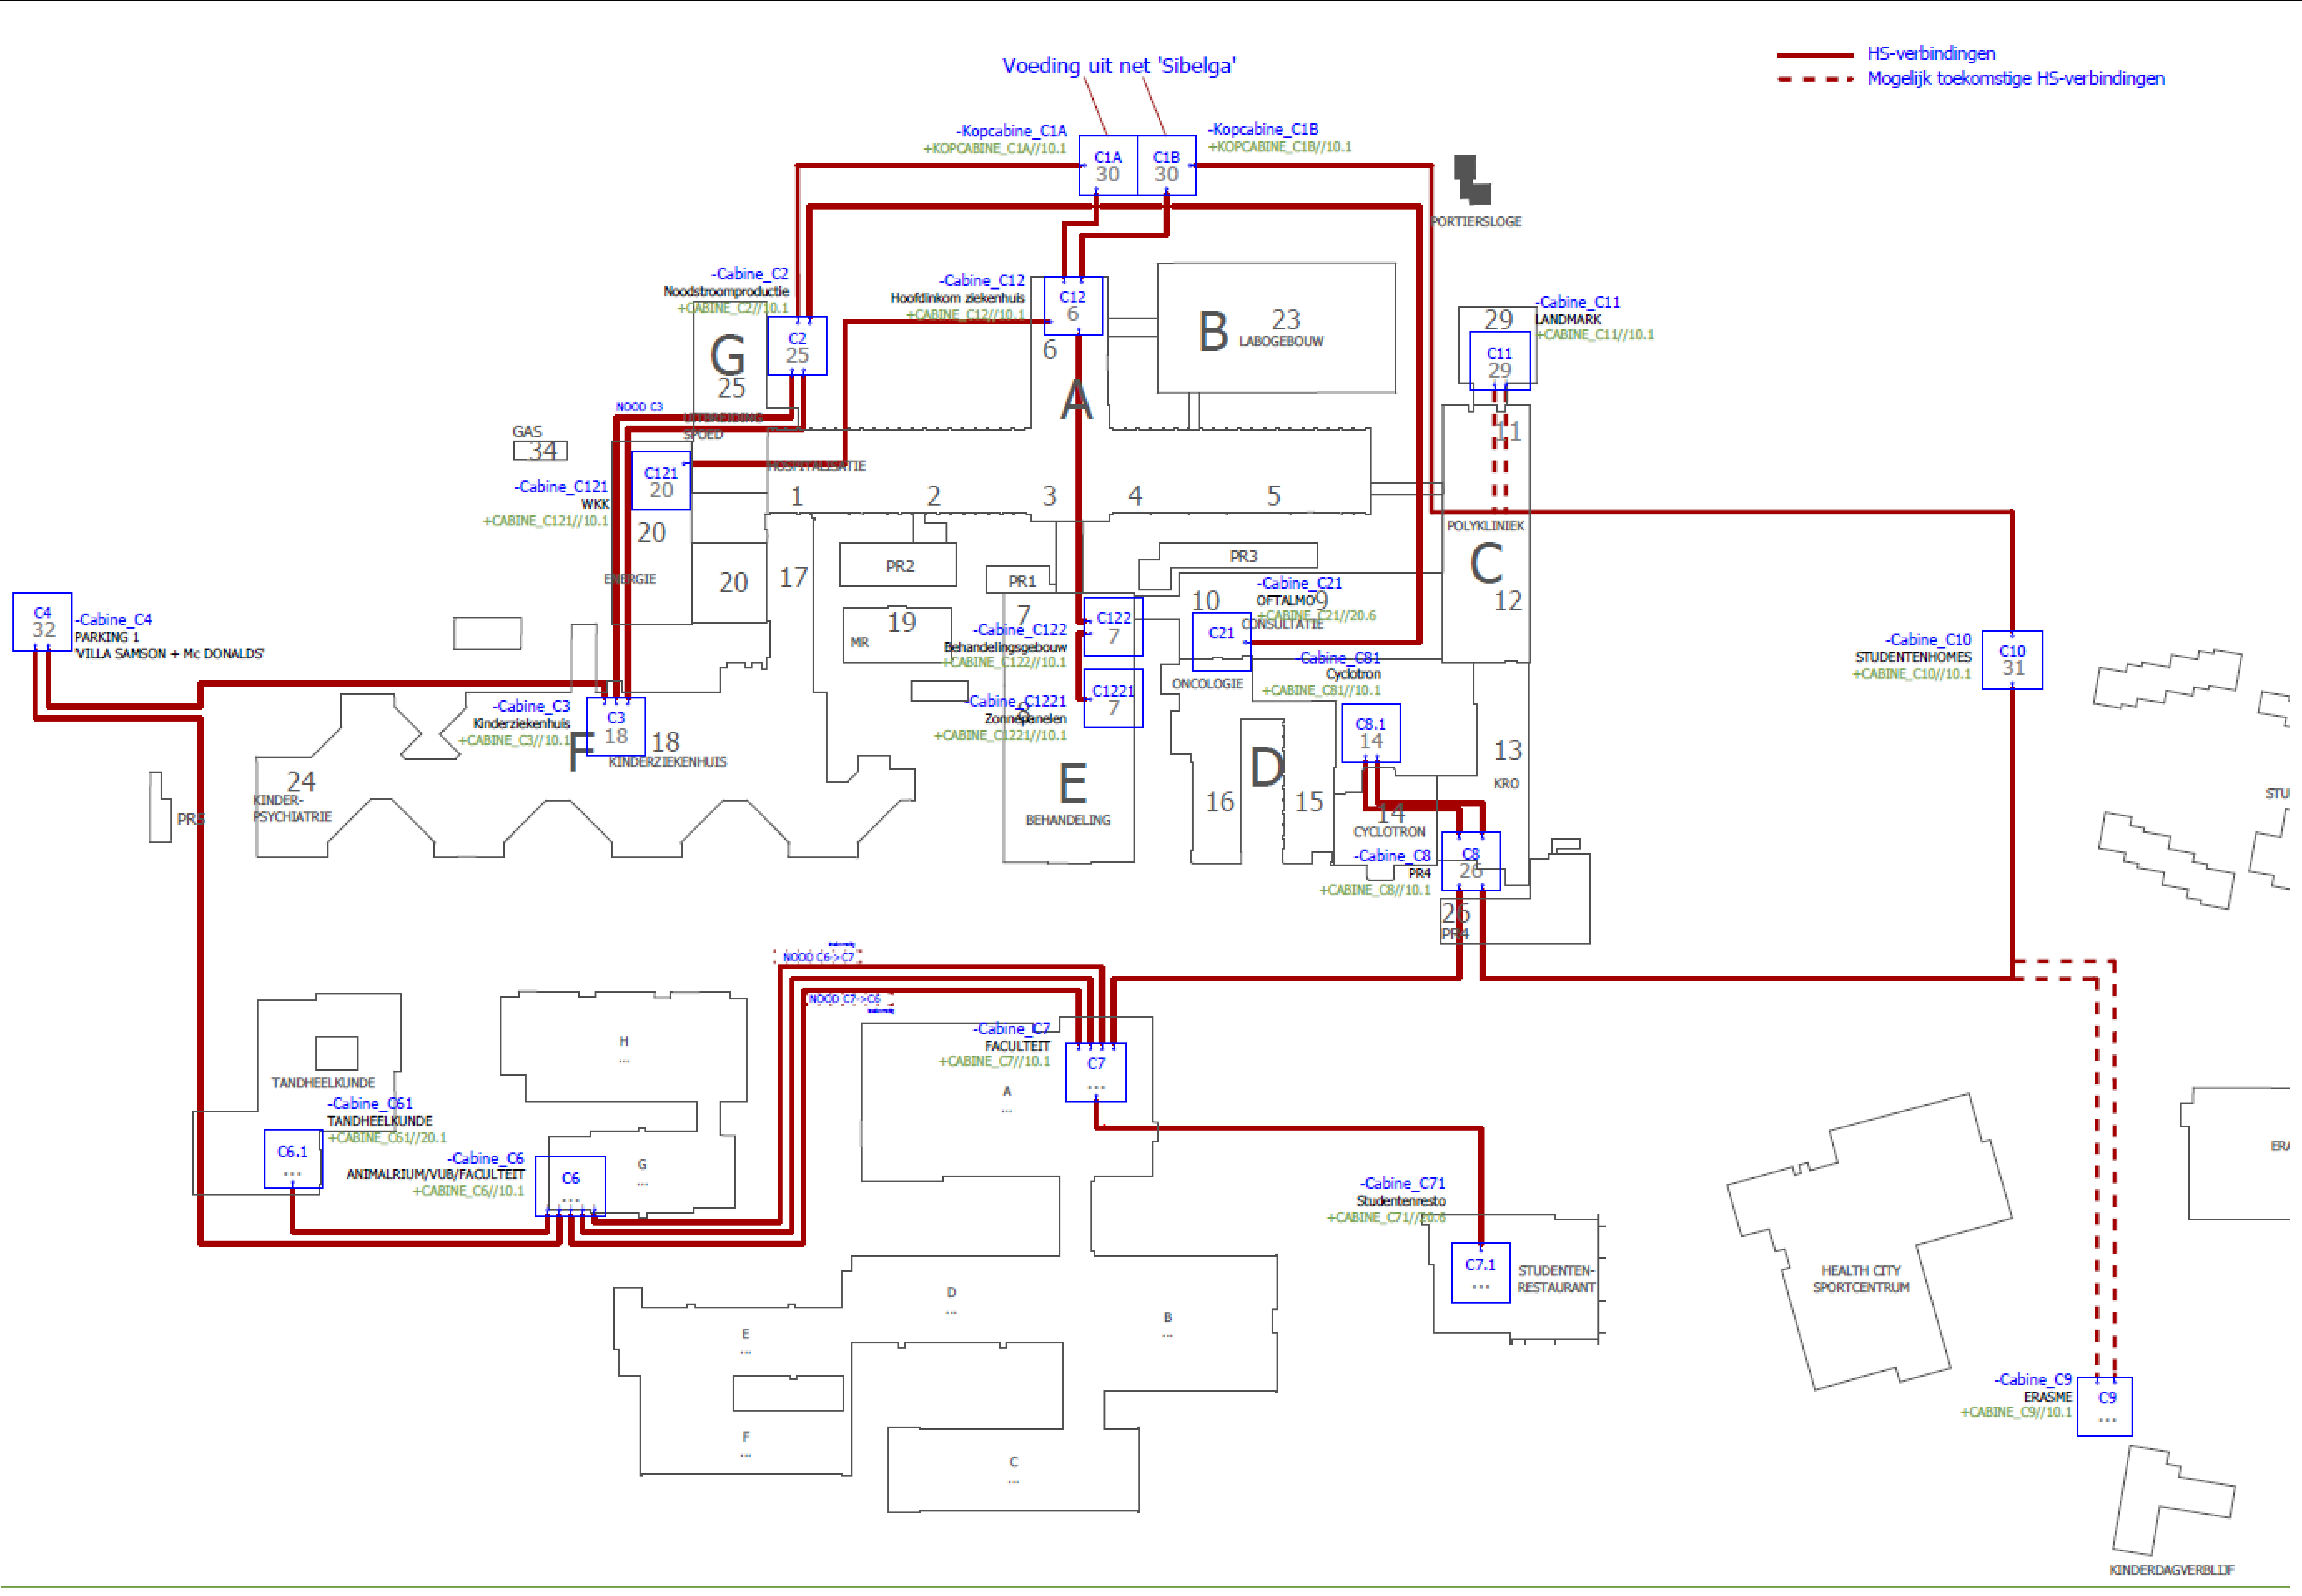
\includegraphics[width=\textwidth]{vub/context/campus_site_layout.pdf}
    \caption{\acs{UZB} electricity distribution network layout}
    \label{fig:bhc_site_layout}
\end{figure}
As part of this project the \ac{BHC}, containing the academic hospital, is a well-advanced
energy island owning and running a state-of-the-art micro-grid that can work in island mode for five consecutive days. 
It includes a thermal and electricity grid, wastewater recovery, a high-
speed glass-fibre telecom network and a total of 33 \ac{HV} transformers divided over 18 \ac{HV} substations.
Energy production and storage includes solar PV, \ac{CHP}, three emergency diesel generators,
and a total capacity of 2,5 MWh in battery storage, mainly under the form of UPS.
The micro-grid serves the hospital complex, 250 student dwellings, the faculty of health
sciences, a primary school and a fitness centre. 
\begin{wrapfigure}{l}{.25\textwidth}
    \centering
    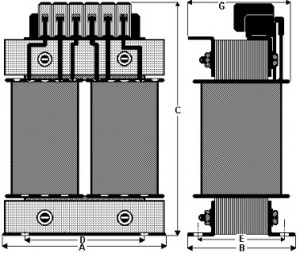
\includegraphics[width=.25\textwidth]{vub/context/trasformatori-uso-sopedaliero-300x253.jpg}
    % \caption{Example of an hospital transformer}
    % \label{fig:transformer_example}
\end{wrapfigure}
The micro-grid system is conceived to go in island mode with complete automatic transition in maximum 15 seconds 
in case of critical need and in three minute to comfort need. 
Cutting edge control technology and maximal reliability are the focus points of this demonstration site.
The hospital, our primary focus, has its own distribution network, as shown in Figure \ref{fig:bhc_site_layout}.
The topology of the network presents a closed-ring shape for increased reliability and is connected to the grid 
through two links to nodes C1A and C1B, located at the same place. Each ``node'' of the network is \ac{HV} cabin identified by a code \{C1, C2, \dots, C12\}, with a main transformer.
Furthermore it can have connection with one or more ``sub'' transformers, like the one showed in before, 
who in turn are connected to ``consumers'' or power sources. These can vary from an individual room to a whole medical department.
% or substations

\subsection{Goal(s), purpose \& critical factors}
\paragraph{Long term}
\begin{itemize}
    \item[$\circledcirc$] Grow Zensor into the main data hub for the Green Energy Park.
    \item[$\circledcirc$] Minimizing the energy losses and overall consumption, leading to a more profitable operation.
    \item[$\circledcirc$] Identify where the exact sources of this cost are and where the best opportunities for improvement lie.
\end{itemize}
\paragraph{Short term}
\begin{itemize}
    \item[$\circledcirc$] Having a view on the data, centralized and well accessible for multiple people in a structured way.
    \item[$\circledcirc$] Monitoring and tracking energy consumption in a production site resulting in more than mere energy bill reductions.
    \item[$\circledcirc$] Improve sustainability reducing energy need and peek request. 
\end{itemize}

\subsection{Project description by phases}
\begin{figure}[ht]
    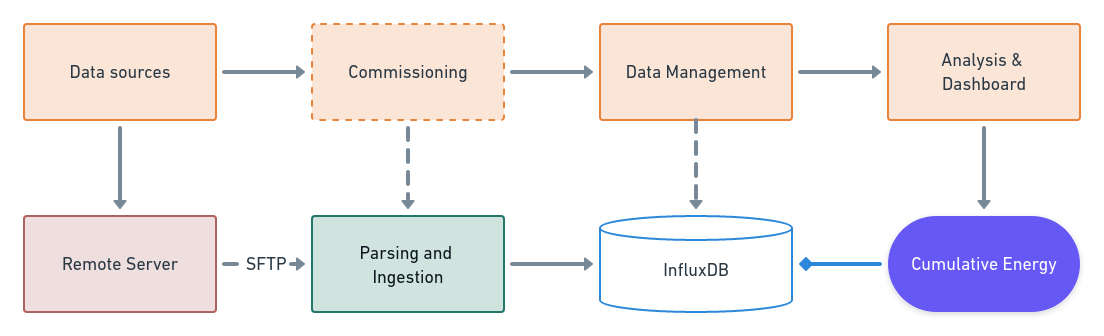
\includegraphics[width=\textwidth]{vub/flowcharts/4_phases.png}
    \caption{\ac{VUB}'s (light) project core stages}
    \label{fig:vub_stages}
\end{figure}

% In this specific project the energy (related parameters) metered at the VUB BHC (the academic hospital in Jette) will have to be stored in our database and visualized for the client. 
% All the 'items' at that point should also have a link to the manual, spec-sheet... of the component (link to Snipe-It or other database).

\paragraph{Datasources}
\begin{figure}[ht]
    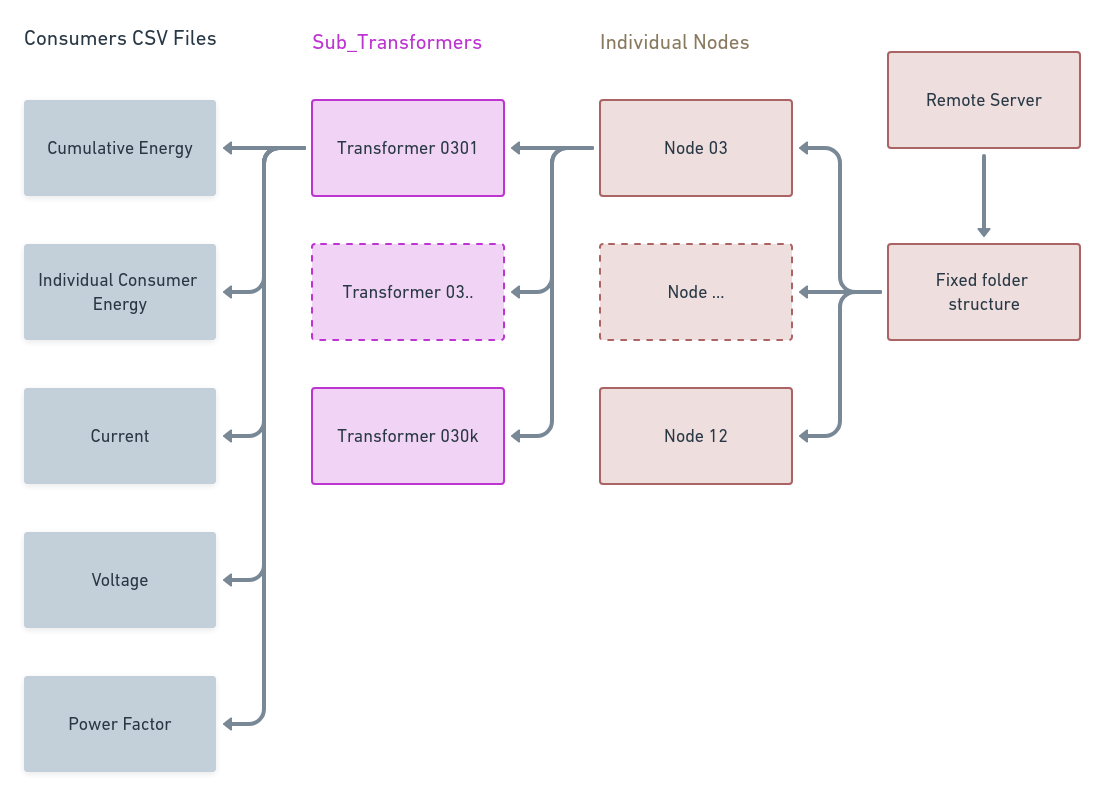
\includegraphics[width=\textwidth]{vub/flowcharts/folder_tree.png}
    \caption{\ac{VUB}'s remote server folder tree structure}
    \label{fig:vub_folder_tree}
\end{figure}
MOBI, \ac{VUB} research group, has collected through the years several MB of 15-minute data energy related out of the distribution network.
This limited dataset is currently stored on a remote server in a simple, yet effective way. 
a folder tree, that tries to reflect reality, is our main metadata's source. 
Looking at Figure \ref{fig:vub_folder_tree} from right to left, in a bottom up manner, should help us clarify the situation. %magari aggiungere colori ai nomi dei diversi livelli come in figura
Starting from the leaves, we found the ``\ac{csv} Files''. Each file share the same common structure with two columns, \textit{time} and \textit{value}, and multiple rows chronologically sorted.
It can either contain information about a secondary transformer or a consumer/power-source as mentioned before in Subsection \ref{sub:vub_initial_hp}. 
To make such distinction we have to rely on his filename, indicating the hardware source and/or the physical element measured.
For example we could find the \texttt{Transfo-I3.csv}, referring to transformer's 3° phase current or \texttt{Bord LG 03 Radiologie.csv} radiology department energy consumption.
How are the different physical quantities organized? To answer this question we go up one level in the tree, moving to the right, stepping up to ``Measurements''. 
Here we have five separated directory. These represent different electricity measurement $\{current, voltage, power\-factor, energy\}$, taken on the secondary \ac{LV} terminals of the transformers. 
About the energy (kWh): we have to make an important distinction between individual or cumulative. It can either represent the consumption of one individual consumer or the whole sub transformer 
(ideally it should be the sum of all consumer connected to it).
Instead, for the others (current, voltage e power factor data later added to the dataset), is only available at the sub transformer level, not consumer. Let's now change the way we traverse the tree, from bottom-up to top down.
From the root (``Fixed folder structure'') we go down to the ``Individual Nodes'' layer, which is pretty self-explanatory. We find in fact a directory for each node of our distribution network. 
This folder contains one or more sub-folder, one for each sub-transformer connected to the same node. Going down even further to the ``Sub transformer'' level, same logic applies. For each sub transformer we have it's one metrics folders.
So here it is the connection point.
To clarify, let's take the previous example and extend it further: the \texttt{Bord LG 03 Radiologie.csv} will have the following path \textit{root/NodeC03/Transfo0302/ConsumerEnergy/Bord\dots}.
%So each set of voltage-files is grouped in to a folder

\paragraph{Commissioning \& Data Management}
% Spostare i dati da un server all'altro e digerirli
\begin{figure}[ht]
    \includegraphics[width=\textwidth]{vub/flowcharts/data-management.png}
    \caption{\ac{VUB}'s data ingestion flowchart}
    \label{fig:vub_ingestion}
\end{figure}
Once the university granted the credential to remotely access this dataset, we started managing it, periodically accessing it using \ac{SFTP} over port 9921. % that is periodically
The \textbf{first step} of the ingestion is, as illustrated in the figure \ref{fig:vub_ingestion}, copying data from \ac{VUB}'s server to Zensor's one. 
This happens periodically as cron job, see Section \ref{subsection:script_structure}, also thanks to Python library \texttt{pysftp}. %enumerate?
We recursively traverses the sftp folder and if we comes across a .csv file we copies it into the same folder structure as on the server.

Subsequently, for \textbf{step two}, we close the connection and work with our freshly copied data. We traverse, once again, the folder tree, keeping track of
folder names that are gonna be important as metadata. Once we are at leaf level, see once again Figure \ref{fig:vub_folder_tree}, we use 
Pandas (\ref{section:pandas}) for file reading, inferring the datetime strings format. This switch to a faster parsing method can increase the speed by 5-10x. %parsing
Then we can perform some data cleaning, for eliminating outliers, duplicates and NaNs.
Immediately afterwards we tag the respective \textbf{DataFrame} with the necessary information to easily identify it, like description, unit and the metadata previously collected.

Since the numerous files are of significant size, this series of operations can take a long time. Therefore, it was decided to parallelize the whole operation using a pool of processes over threads.
To substantiate this point, here is a small digression: 
in Python, if code is CPU-bound, multithreading won't help, because only one thread can hold the Global Interpreter Lock, and therefore run Python code, at a time. 
So, in this specific scenario we need to use processes, not threads. Indeed in multiprocessing, any newly created process will run independently with its own memory space.

Finally, the \textbf{step three} involves writing each DataFrame on the InfluxDB (\ref*{section:influxdb}), our choice for \acl{tsdb}.
This operation, which is already quite optimized, can be easily executed in parallel given the limited concurrency.
As a result we will have a ``measurement'' for each node, which will contain several series, each one easily distinguishable from the others.

\paragraph{Analysis}
\begin{figure}[ht]
    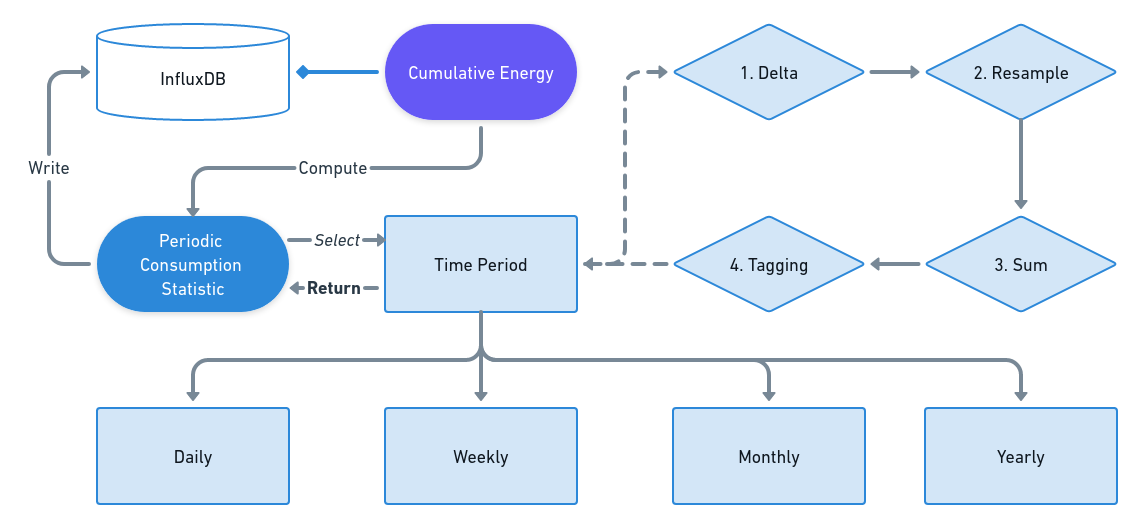
\includegraphics[width=\textwidth]{vub/flowcharts/analystic_flowchart.png}
    \caption{\ac{VUB}'s analytics chart}
    \label{fig:vub_anal_chart}
\end{figure}
They want to see some basic visualizations of this limited dataset, no live link or permanent ingestion will have to be set up.
In a first instance the dashboards need to have the same structure as the folders the .csv files are in.
So: each folder containing .csv files should be a page in Grafana displaying the graphs of the series inn the .csv's in that folder.
In a second instance they want the entry point to be a map of the campus with the main transformers indicated and with a clickable link on each item such that the data can be consulted. 


\subsection{Conclusion}
